\documentclass[11pt]{article}
\usepackage{geometry}
\geometry{a4paper}
\usepackage[parfill]{parskip}
\usepackage{graphicx}
\usepackage{amssymb}
\usepackage{epstopdf}
\usepackage{fancyhdr}
\usepackage{fullpage}
\usepackage{appendix}
\usepackage{newclude}
\usepackage{datetime}
\usepackage{hyperref}
\usepackage{breakurl}
\usepackage{color}
\usepackage{multind}
\usepackage{microtype}
\usepackage{tabularx}
\usepackage{fancybox}

\makeindex{pve}
\newcommand{\pve}[1]{ }
\newcommand{\pvelist}[1]{  }

\makeindex{drupalpath}
\newcommand{\drupalpath}[1]{\index{drupalpath}{#1}\url{gemeente.nl/#1}}

\hypersetup{
    colorlinks,
    citecolor=black,
    filecolor=black,
    linkcolor=black,
    urlcolor=black
}

\DeclareGraphicsRule{.tif}{png}{.png}{`convert #1 `dirname #1`/`basename #1 .tif`.png}

\newcommand{\seeone}[1]{ (zie \ref{#1} p.\pageref{#1})}
\newcommand{\seetwo}[2]{ (zie \ref{#1} p.\pageref{#1},  \ref{#2} p.\pageref{#2})}

\pagestyle{fancy}
\fancyhead{}
\fancyfoot{}
\fancyfoot[R]{\thepage}

\setcounter{secnumdepth}{5}
\setcounter{tocdepth}{5}

\makeatletter
\renewcommand\paragraph{%
   \@startsection{paragraph}{4}{0mm}%
      {-\baselineskip}%
      {.5\baselineskip}%
      {\normalfont\normalsize\bfseries}}
\makeatother

\newcommand{\customer}{Dimpact}
\newcommand{\thecustomer}{\customer}
\newcommand{\customerdomain}{schijndel.nl}
\newcommand{\customerdomainuc}{Schijndel.nl}

\title{Training \customer \\ \customerdomainuc}
\author{David van Dijk}
\date{}

\begin{document}
\maketitle
\begin{center}

Laatst bijgewerkt: \\ \ddmmyyyydate \today
\end{center}
\pagebreak

\renewcommand*\contentsname{Inhoudsopgave}
\tableofcontents
\pagebreak

Voor alle onderstaande cases dient er ingelogd te zijn met een gebruiker met de juiste rechten. Op sommige afbeeldingen zullen meer onderdelen te zien kunnen zijn dan waar je toegang tot hebt. 

Met de adminbalk wordt de zwarte balk bovenaan de website bedoeld die ten alle tijden zichtbaar is wanneer men is ingelogd met een gebruiker met de juiste rechten.

\section{Toevoegen van content}

\subsection{Nieuws toevoegen}

\begin{enumerate}
\item Ga met je muis in de adminbalk op \emph{Mijn Workbench} staan. Beweeg je muis dan over \emph{Inhoud aanmaken}.
\item Kies dan \emph{Nieuws} uit de lijst met content types die dan verschijnt.

\begin{center}
	\shadowbox{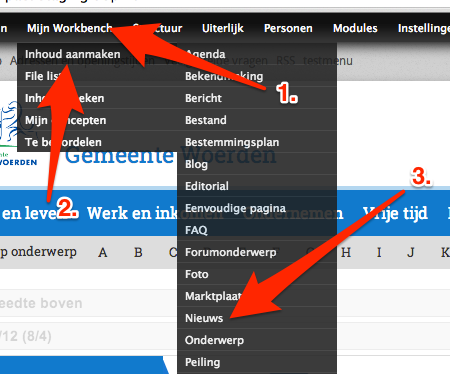
\includegraphics[scale=0.5]{img/addcontent.png}}
\end{center}

\item Het volgende scherm zal het content bewerkscherm zijn.

\begin{center}
	\shadowbox{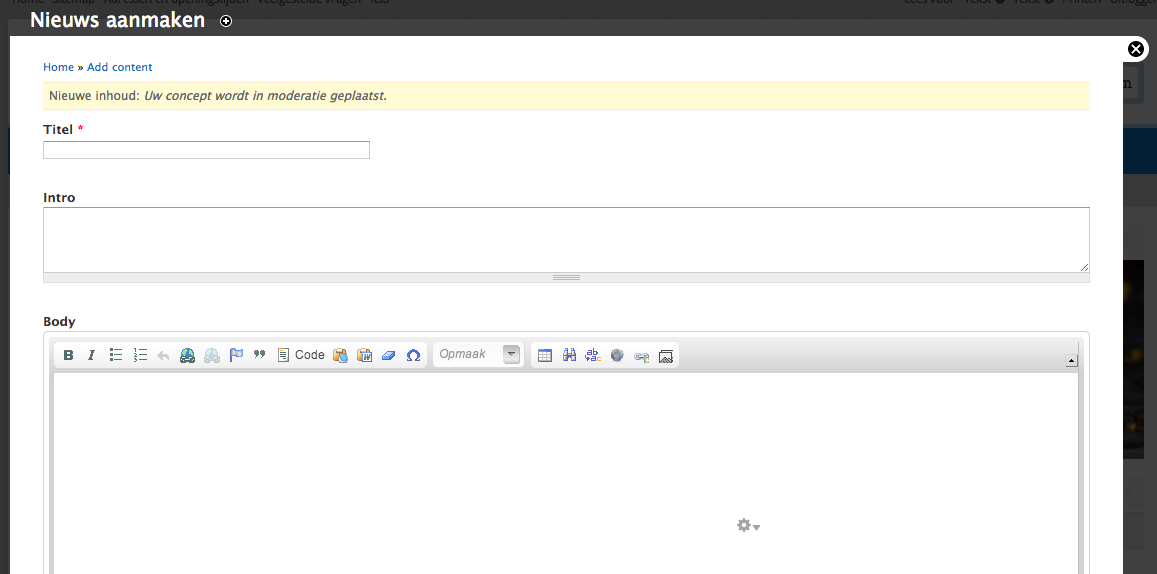
\includegraphics[scale=0.3]{img/addnews.png}}
\end{center}

\item Vul de volgende velden in \emph{Titel (verplicht)}, \emph{Intro}, \emph{Body}, \emph{Image}, \emph{Tags}, \emph{Locatie}.
\item Laat de overige velden zoals ze zijn en druk op \emph{Opslaan}.
\end{enumerate}

Na het opslaan kom je terecht op het zojuist aangemaakte nieuwsitem. Herhaal deze stap om meerdere nieuwsberichten aan te maken. Dit nieuwsbericht is opgeslagen als concept en zal als concept terug te vinden zijn in je \emph{Workbench}.

\section{Beheren van content (Workbench)}

\begin{enumerate}
\item Klik op \emph{Mijn Workbench} in de adminbalk. Je komt nu terecht op de voorpagina van je workbench.

\begin{center}
	\shadowbox{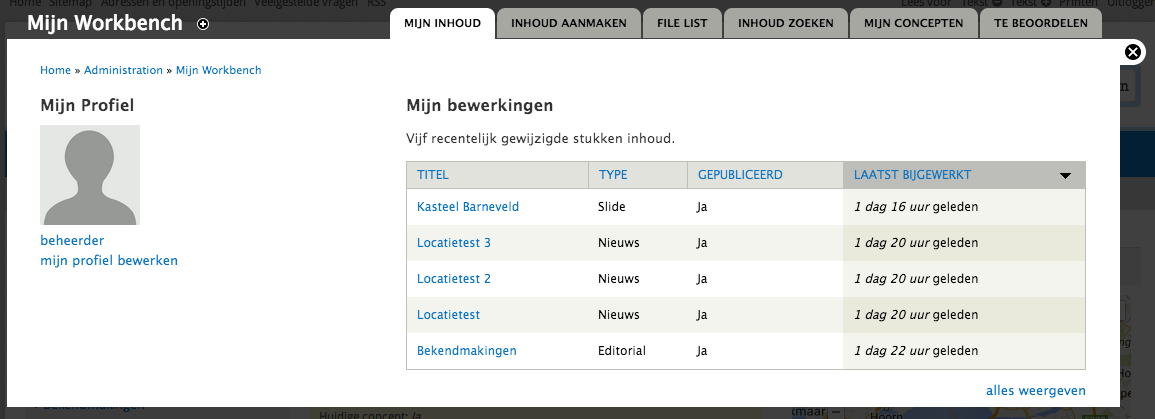
\includegraphics[scale=0.3]{img/workbench.png}}
\end{center}

\item Je ziet nu een lijst met de vijf meest recent gewijzigde contentitems. Daartussen staat het zojuist aangemaakte nieuwsbericht. Deze staat op niet gepubliceerd.
\item Ga naar het tabblad \emph{Mijn concepten}.
\item Klik bij het juiste item in de lijst op \emph{Wijzig naar Ter beoordeling}. Het nieuwsbericht is nu gekenmerk als \emph{Te boordelen} en kan door een eindredacteur gepubliceerd worden. In deze lijst staat \emph{alleen} content die je \emph{zelf} aangemaakt hebt. 
\item Klik als eindredacteur op het tabblad \emph{Te beoordelen}.
\item Klik op \emph{Wijzig naar concept} om het item terug te zetten naar concept voor de (eind)redacteur. Klik op \emph{Wijzig naar Gepubliceerd} om het item te publiceren en zichtbaar te maken op de website.
\end{enumerate}

\section{Pagina aanmaken}\label{nieuwepagina}

Hiervoor dient ingelogd te zijn als beheerder, of de eerste 5 stappen moeten zijn uitgevoerd door een beheerder. Vanaf stap 6 kan verder worden gewerkt wanneer de pagina bestaat.

\begin{enumerate}
\item Klik op \emph{Empty Page callbacks} onder \emph{Structuur}.
\begin{center}
	\shadowbox{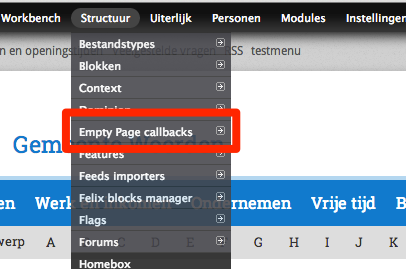
\includegraphics[scale=0.5]{img/epcb.png}}
\end{center}
\item Klik op het tabblad \emph{Add callback}
\item Vul bij Intern pad "\textbf{nieuws}" in en laat de titel leeg.
\item Druk op \emph{Toevoegen}. Je komt nu terug op de overzichtspagina.
\item Druk op \emph{Weergeven} naast nieuws. Je komt nu op een lege pagina (/nieuws) terecht.
\begin{center}
	\shadowbox{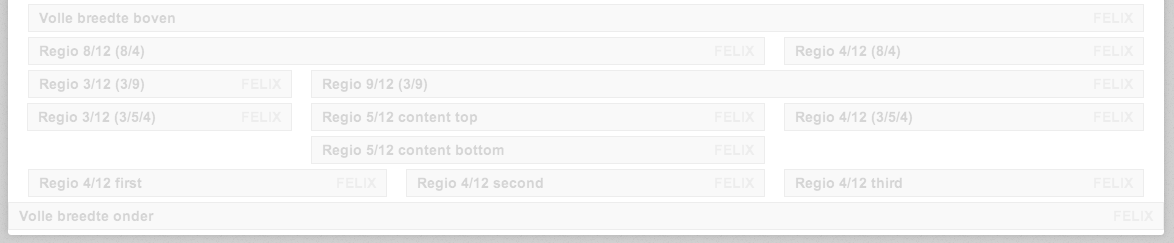
\includegraphics[scale=0.3]{img/emptyfelix.png}}
\end{center}
\item Plaats de muis op \emph{Regio 5/12 content top} en druk het op tandwiel. Selecteer dan \emph{Blok toevoegen}.
\begin{center}
	\shadowbox{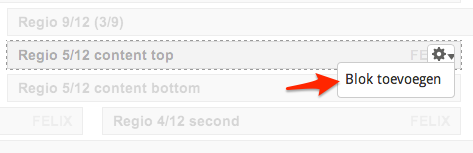
\includegraphics[scale=0.5]{img/addblock.png}}
\end{center}
\item Kies dan \emph{Nieuws teaserblok}.
\begin{center}
	\shadowbox{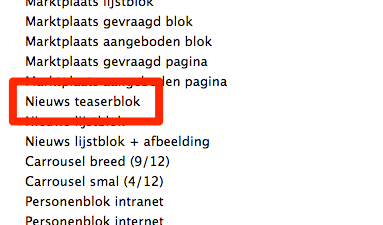
\includegraphics[scale=0.5]{img/selectblock.png}}
\end{center}
\item Vul bij \emph{Onderwerp} "\textbf{Nieuws}" in.
\item Druk op \emph{Opslaan}. Je gaat nu terug naar de pagina met het zojuist toegevoegde blok.
\item Vul de rechterkolom met de \emph{Agenda lijstblok} in de regio \emph{Regio 4/12 (3/5/4)}.
\end{enumerate}

\subsection{Onderwerpenpagina maken}

\begin{enumerate}
\item Maak een nieuw content item aan van het type \emph{Onderwerp}.
\item Vul een titel in.
\item Laat de body leeg.
\item Selecteer het tabblad \emph{URL-pad-instellingen}.
\item Zet het vinkje bij \emph{Automatische URL-alias aanmaken} uit.
\item Vul bij \emph{URL-alias} een korte url in, bijvoorbeeld "\textbf{wonen-en-leven}" of "\textbf{werk-en-inkomen}".
\item Selecteer het tabblad \emph{Reactie-instellingen} en controleer of deze op gesloten staat.
\item Ga dan naar /wonen-en-leven (of een andere url opgegeven bij de vorige stap). In de volgende stappen maken we blokken aan die we op deze pagina neerzetten.
\item Maak een nieuw content item aan van het type \emph{Editorial}.
\item Geef een titel op en vul de body.
\item Selecteer een pictogram bij \emph{Foto} om een afbeelding in de titel van het blok te zetten.
\item Sla op.
\item Ga naar /\emph{wonen-en-leven} (of de url die aangemaakt is bij de vorige stappen.
\item \emph{Blok toevoegen} in een van de volgende regio's; \emph{Regio 4/12 first}, \emph{Regio 4/12 second} of \emph{Regio 4/12 third}.
\item Kies dan onder \emph{Nodetype}: "\textbf{Editorial}".
\begin{center}
	\shadowbox{
\includegraphics[scale=0.5]{img/addeditorial.png}}
\end{center}
\item Selecteer dan \emph{Volledige inhoud}.
\item Zoek of selecteer dan de content die bij stap 1 is aangemaakt. Op de titel drukken is voldoende om het blok in de regio te zetten.
\item Je gaat automatisch terug naar de pagina met het blok in de gekozen regio.
\end{enumerate}

\section{Pagina koppelen als menuitem}

\subsection{Hoofdmenuitem}

\begin{enumerate}
\item Ga naar \emph{Structuur} - \emph{Menu's}
\begin{center}
	\shadowbox{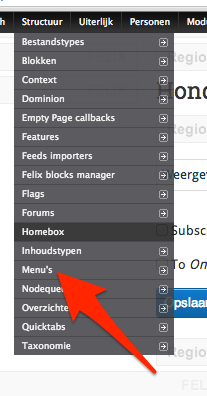
\includegraphics[scale=0.5]{img/menus.png}}
\end{center}
\item Druk op \emph{links weergeven} bij \emph{Main menu}.
\item Druk op \emph{Link toevoegen}.
\item Vul een titel in bij \emph{Titel van menulink}.
\item Vul bij het pad "\textbf{wonen-en-leven}" in (of een ander pad gebruikt bij de vorige stappen).
\item Zet de optie \emph{Uitgeklapt weergeven} aan.
\item Druk op \emph{Opslaan}.
\item Ga naar de voorpagina (of een andere willekeurige pagina) en controleer of er een menuitem bij is gekomen.
\end{enumerate}

\subsection{Submenuitem}

\begin{enumerate}
\item Ga naar \emph{Structuur} - \emph{Menu's}
\begin{center}
	\shadowbox{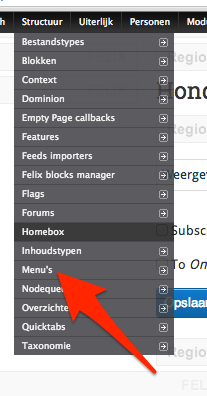
\includegraphics[scale=0.5]{img/menus.png}}
\end{center}
\item Druk op \emph{links weergeven} bij \emph{Main menu}.
\item Druk op \emph{Link toevoegen}.
\item Vul een titel in bij \emph{Titel van menulink}.
\item Vul bij het pad, het pad in wat gebruikt was om een nieuw pagina te maken \emph{Pagina aanmaken}\seeone{nieuwepagina}.
\item Selecteer bij \emph{Bovenliggend onderdeel} een menuitem op het eerste niveau (zie screenshot). Je kan het item gebruiken wat bij het vorig onderdeel is aangemaakt.
\begin{center}
	\shadowbox{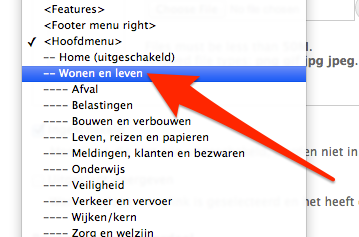
\includegraphics[scale=0.5]{img/submenu.png}}
\end{center}
\item Sla het menuitem op.
\item Ga naar de voorpagina (of een andere willekeurige pagina) en controleer of er een submenuitem bij is gekomen.
\end{enumerate}

Als je hebt gekozen voor de /nieuws pagina zal je zien dat er een blok aan de Linkerkant bij is gekomen. Deze heeft als titel de naam van het hoofdmenuitem. Daaronder vallen de submenuitems en subsubmenuitems.

Voor het aanmaken van subsubmenuitems volg je dezelfde stappen maar geef je een menuitem op als bovenliggend onderdeel, dat een niveau dieper ligt (zie screenshot)
\begin{center}
	\shadowbox{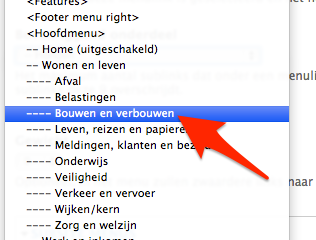
\includegraphics[scale=0.5]{img/subsubmenu.png}}
\end{center}

\section{Carrousel bewerken (nodequeue's)}

\begin{enumerate}
\item Maak een nieuw content item aan van het type \emph{Slide}.
\item Vul een titel in.
\item Link invullen is optioneel.
\item Selecteer een afbeeldingen onder \emph{Image}. Let op dat deze van dusdanige kwaliteit en grootte moet zijn dat hij minstens 738 pixels breed is.
\item Laat de body leeg.
\item Selecteer bij \emph{Publicatie-opties} moderatiestatus: Gepubliceerd. Of laat dit doen door een eindredacteur.
\item Herhaal dit een paar keer om meerdere slides te maken.
\item Ga naar \emph{Structuur} - \emph{Nodequeues}
\begin{center}
	\shadowbox{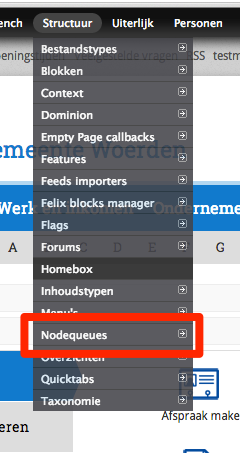
\includegraphics[scale=0.5]{img/nodequeues.png}}
\end{center}
\item Druk op \emph{Weergeven} bij \emph{Carousel 9/3}.
\item Vul in het zoekveld onderaan de lijst de titel van een slide in.
\item Selecteer een gevonden slide en druk op \emph{Inhoud toevoegen}.
\item Pas de volgorde van de slides aan via het sleepicoon links van de titels.
\item Verwijder slides door op \emph{verwijderen} te drukken.
\item Druk op \emph{Opslaan}.
\end{enumerate}
\clearpage

\end{document}
